% ============================================================================
% TP Sistemas de Computación – Informe completo
% Índice GINI + Python + C (32 bits) + Ensamblador NASM + GDB
% ============================================================================
\documentclass[a4paper,12pt]{article}
\catcode`\_=12
% ----------------------- Paquetes básicos ----------------------------------
\usepackage[utf8]{inputenc}
\usepackage[T1]{fontenc}
\usepackage[spanish]{babel}
\usepackage{graphicx}
\usepackage{subcaption}
\usepackage{caption}
\usepackage{listings}
\usepackage{amsmath}
\usepackage{float}
\usepackage{geometry}
\usepackage{fancyhdr}
\usepackage{enumitem}
\usepackage{booktabs}
\usepackage[hidelinks]{hyperref}
\usepackage{cleveref}
\usepackage{xcolor}

% ----------------------- Configuración global ------------------------------
\geometry{margin=2.5cm}
\graphicspath{{images/}}
\pagestyle{fancy}
\fancyhf{}
\lhead{GINI + Python + C + ASM + GDB}
\rhead{TP Sistemas de Computación}
\cfoot{\thepage}

% ----------------------- Listings ------------------------------------------
\lstdefinelanguage{NASM}{
  morekeywords={section,global,extern,fld,fistp,add,leave,ret,push,mov,sub},
  sensitive=true,
  morecomment=[l]{;},
  morestring=[b]",
}
\lstset{
  basicstyle=\ttfamily\small,
  numberstyle=\tiny,
  numbers=left,
  stepnumber=1,
  frame=single,
  captionpos=b,
  keywordstyle=\color{blue},
  commentstyle=\itshape\color{gray!70},
}

% =============================================================================
\begin{document}
\begin{titlepage}
    \begin{center}
        {\LARGE \textbf{Universidad Nacional de Córdoba}}\\[1.5cm]

        
\includegraphics[scale=0.4]{images/logo2.png}\\[1.5cm]

        {\large Facultad de Ciencias Exactas, Físicas y Naturales}\\
        {\large Escuela de Electrónica y Computacion}\\[1cm]

        \rule{\linewidth}{0.5mm}\\[0.4cm]
        {\Large \textbf{Cátedra de Sistemas de Computacion}}\\[0.3cm]
        {\LARGE \textbf{Trabajo de Laboratorio 3}}\\[0.3cm]

        \rule{\linewidth}{0.5mm}\\[1cm]

        \begin{flushleft}
        {\large 
            \textbf{Profesor Titular:} Ing. Javier Alejandro JORGE\\
            \textbf{Profesor Adjunto:} -\\[0.5cm]
            \textbf{Integrantes:}\\
            Trucchi, Genaro\\
            Trachtta, Agustin\\
            Rodriguez, Mateo\\
        }
        \end{flushleft}

        \vfill

        {\large \today}
    \end{center}
\end{titlepage}

\tableofcontents
\newpage

% ---------------------------------------------------------------------------
\section{Objetivos generales}
\begin{itemize}[leftmargin=*]
  \item Consumir una API REST pública (Banco Mundial) para obtener el índice GINI de un país.
  \item Transferir el dato a un módulo intermedio en \texttt{C} compilado en 32 bits.
  \item Llamar, desde \texttt{C}, una rutina de ensamblador NASM que convierta el float a entero y realice una transformación aritmética mínima.
  \item Inspeccionar con \textbf{GDB} la pila (\emph{stack}) antes, durante y después de la llamada, mostrando el cumplimiento de la convención de llamada \emph{cdecl}.
  \item Documentar el flujo end‑to‑end y justificar todas las decisiones de diseño.
\end{itemize}
% ---------------------------------------------------------------------------

\section{Descripción general del funcionamiento}
\begin{figure}[H]
  \centering
  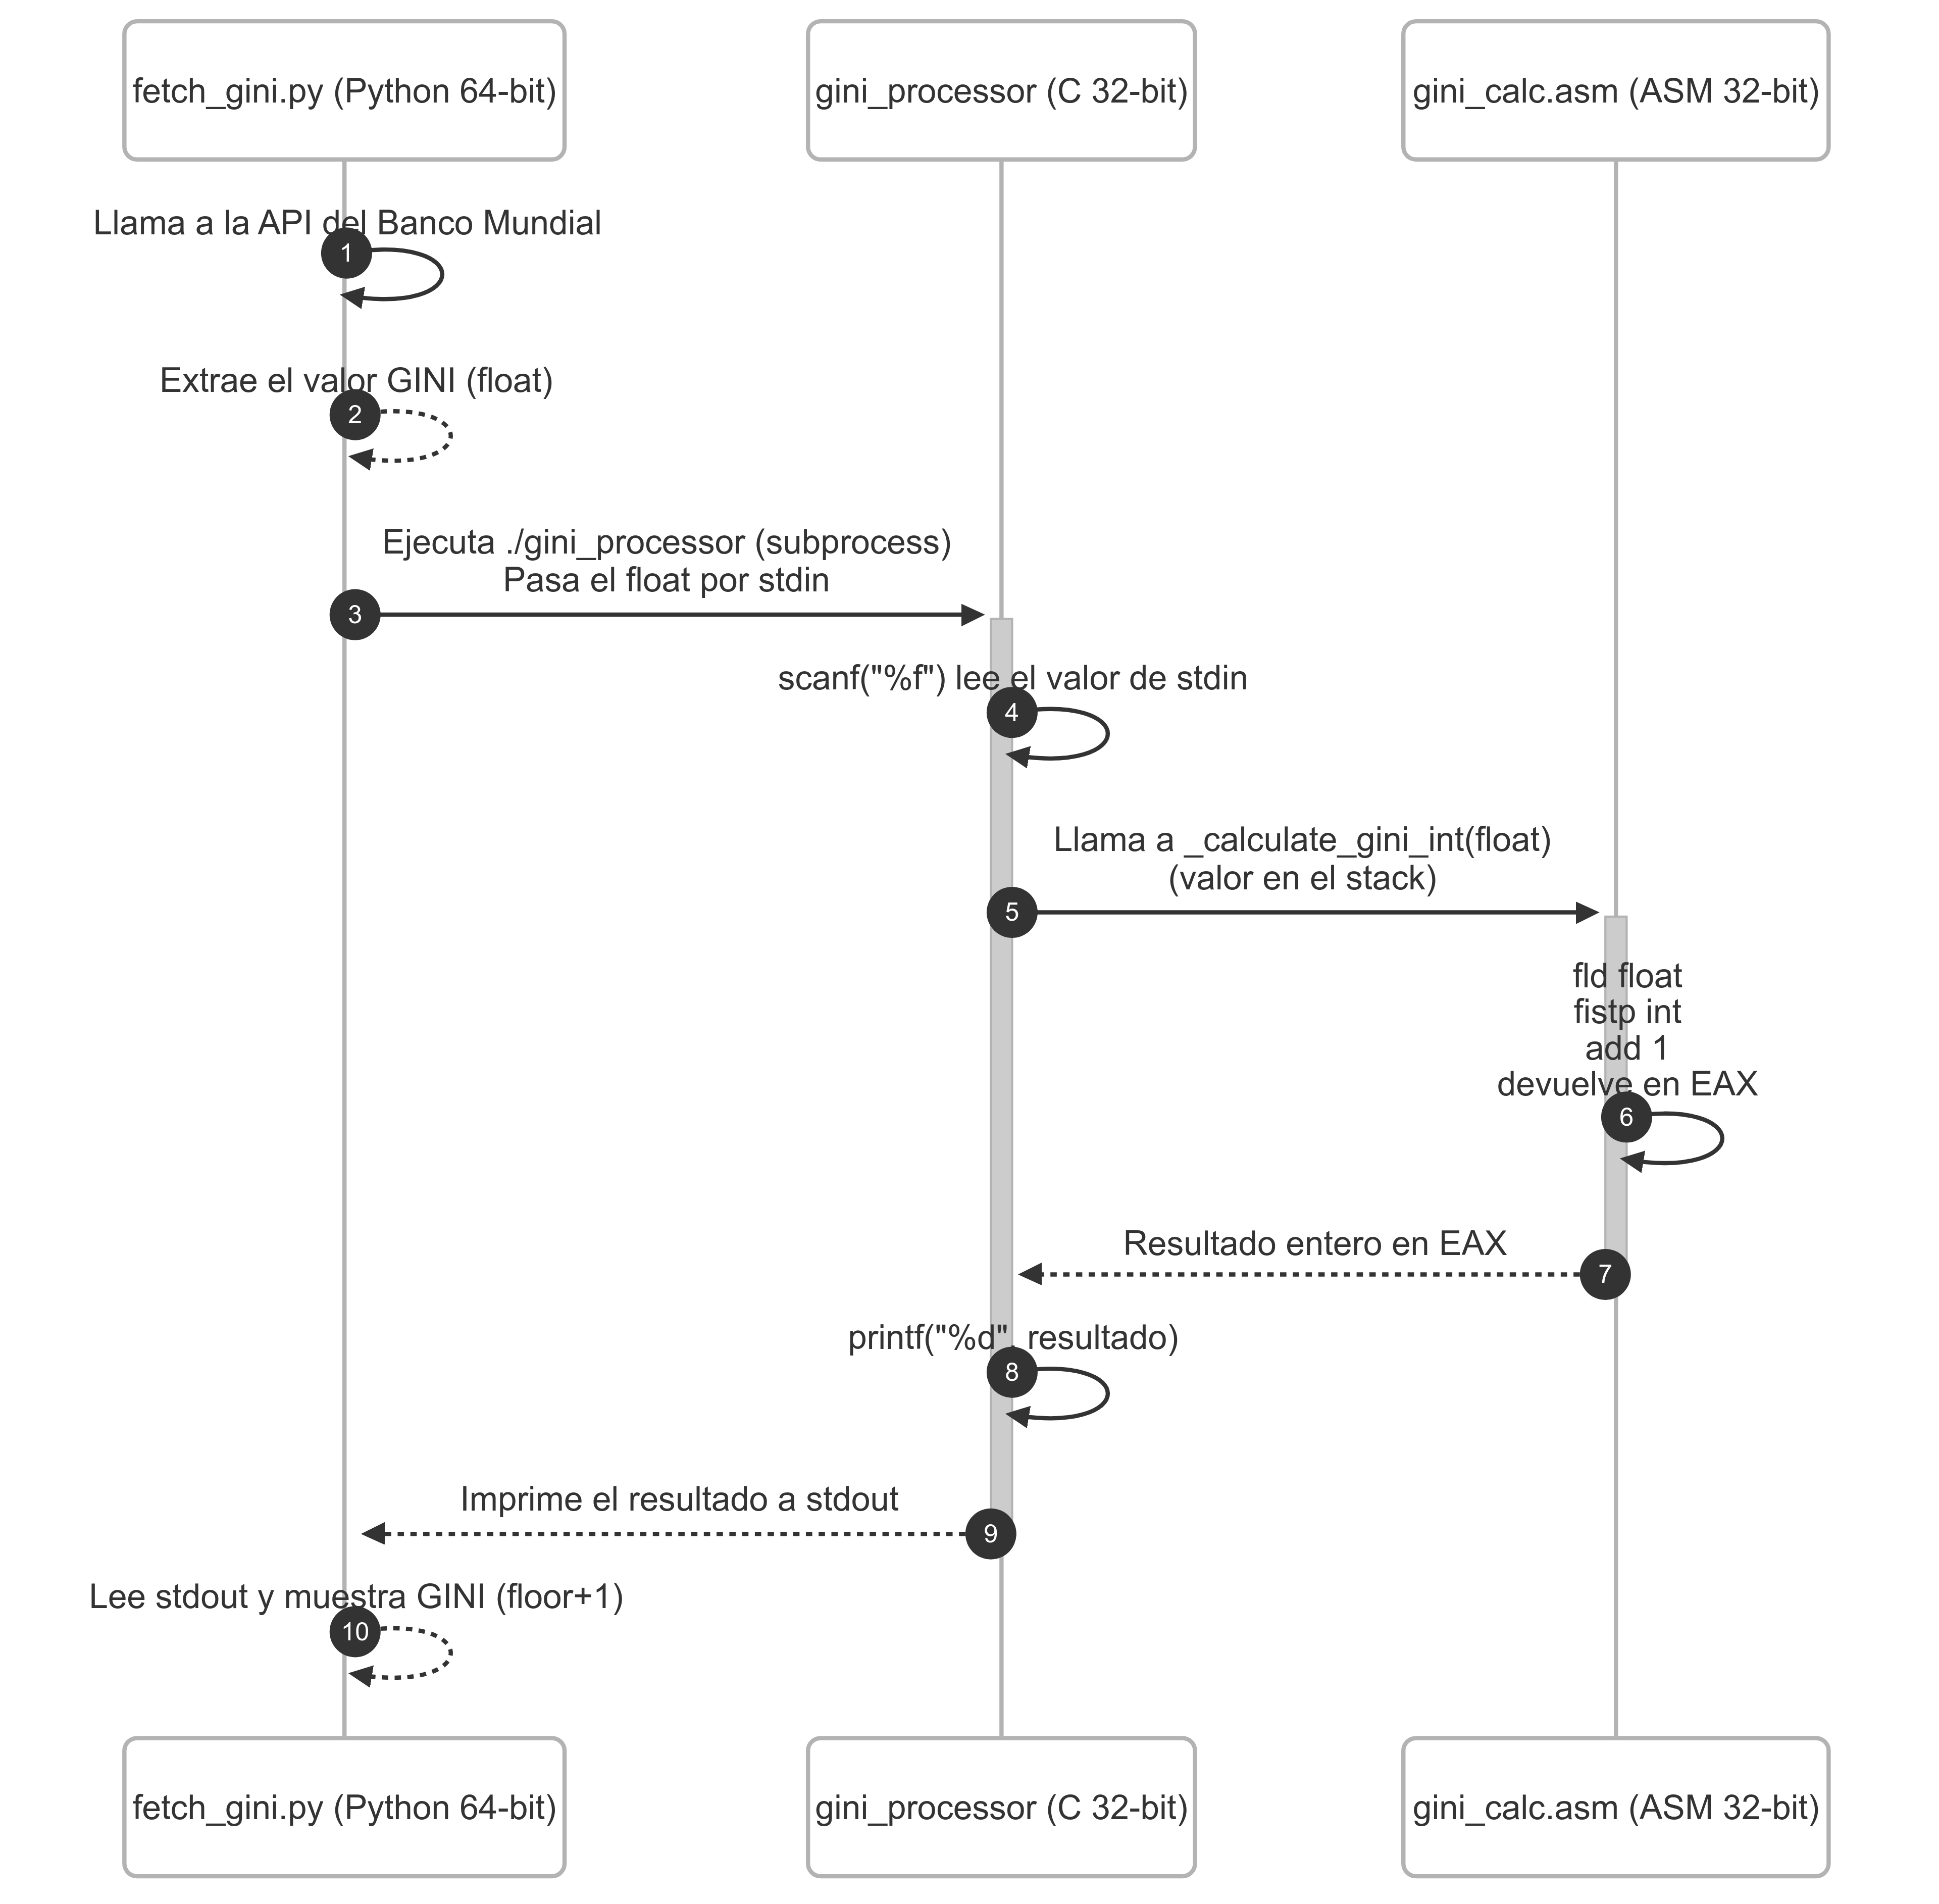
\includegraphics[width=0.85\textwidth]{images/diagram.png}
  \caption{Flujo de ejecución completo: desde la API REST hasta la rutina en ensamblador.}\label{fig:sequence}
\end{figure}

Esta imagen resume cómo interactúan los distintos componentes del proyecto. El flujo se desarrolla de la siguiente manera:

\begin{enumerate}[label=\textbf{\arabic*.}]
  \item El script \texttt{fetch\_gini.py} (escrito en Python 64-bit) realiza una consulta HTTP a la API del Banco Mundial.
  \item Se extrae del JSON el valor GINI más reciente (tipo \texttt{float}).
  \item Python lanza el binario \texttt{gini\_processor} como un subproceso y le pasa el número flotante vía \texttt{stdin}.
  \item El programa en C (compilado en 32-bit) recibe el valor con \texttt{scanf("f")} y lo guarda como variable local.
  \item Luego invoca la función externa \texttt{calculate\_gini\_int(float)}, definida en NASM, pasando el argumento a través de la pila (\texttt{cdecl}).
  \item En la rutina NASM:
    \begin{itemize}
      \item Se carga el \texttt{float} desde \texttt{[ebp+8]} en la FPU con \texttt{fld}.
      \item Se convierte a entero truncado con \texttt{fistp} y se guarda en \texttt{[esp]}.
      \item Se mueve a \texttt{eax}, se le suma 1, y se devuelve a C.
    \end{itemize}
  \item El resultado queda disponible en \texttt{EAX}.
  \item En C, se imprime ese valor con \texttt{printf}.
  \item Python captura la salida estándar del subproceso.
  \item Finalmente, se muestra el resultado por consola, que corresponde a \texttt{floor(GINI) + 1}.
\end{enumerate}

Este diseño evidencia una integración end-to-end desde el consumo de servicios web hasta el uso de bajo nivel del stack y los registros en arquitectura x86.

% ---------------------------------------------------------------------------
\section{Arquitectura de capas y flujo de datos}

\subsection{Motivación de las capas}
\begin{description}[leftmargin=2em]
  \item[Python.] Facilita el consumo de APIs REST gracias a bibliotecas de alto nivel, parsing JSON y scripting rápido.
  \item[C (32 bits).] Puente con el código de bajo nivel; permite compilar con \texttt{-m32} para emular un entorno clásico x86 y simplificar el llamado a NASM.
  \item[Ensamblador NASM.] Exponer al alumno al manejo explícito de registros, FPU y pila; reforzar el concepto de convención de llamada y optimización de bajo nivel.
\end{description}


% ---------------------------------------------------------------------------
\section{API REST: concepto y uso práctico}
\subsection{¿Qué es una API REST?}
Una API REST (\emph{Representational State Transfer}) expone recursos a través de
métodos HTTP estándar (\texttt{GET}, \texttt{POST}, \dots). El servidor devuelve
una representación —en nuestro caso JSON— que el cliente parsea.

\subsection{Banco Mundial – endpoint utilizado}
\begin{lstlisting}[language={},caption={URL solicitada}]
https://api.worldbank.org/v2/en/country/ARG/indicator/SI.POV.GINI?
        format=json&date=2011:2020&per_page=50&page=1
\end{lstlisting}
Parámetros:
\begin{itemize}
  \item \texttt{country=ARG}: Argentina.
  \item \texttt{indicator=SI.POV.GINI}: índice GINI.
  \item \texttt{date=2011:2020}: rango de años.
  \item \texttt{format=json}: respuesta JSON.
\end{itemize}

% ---------------------------------------------------------------------------
% ---------------------------------------------------------------------------
\section{Convención de llamada \emph{cdecl} y la pila}
La convención \emph{cdecl} (``C declaration'') es la que usa por defecto
\texttt{gcc} en x86 para funciones externas.  
Los \textbf{argumentos} se empujan en la pila de \emph{derecha a izquierda};
el \textbf{caller} (quien llama) también es responsable de limpiar esa pila
después del \texttt{call}.  
La callee (\texttt{calculate\_gini\_int} en nuestro caso) arma un marco
(\emph{stack frame}) clásico con \texttt{push ebp} / \texttt{mov ebp,esp}.

% ---------------------------------------------------------------------------
\subsection{Layout del stack frame}
\begin{figure}[H]
  \centering
  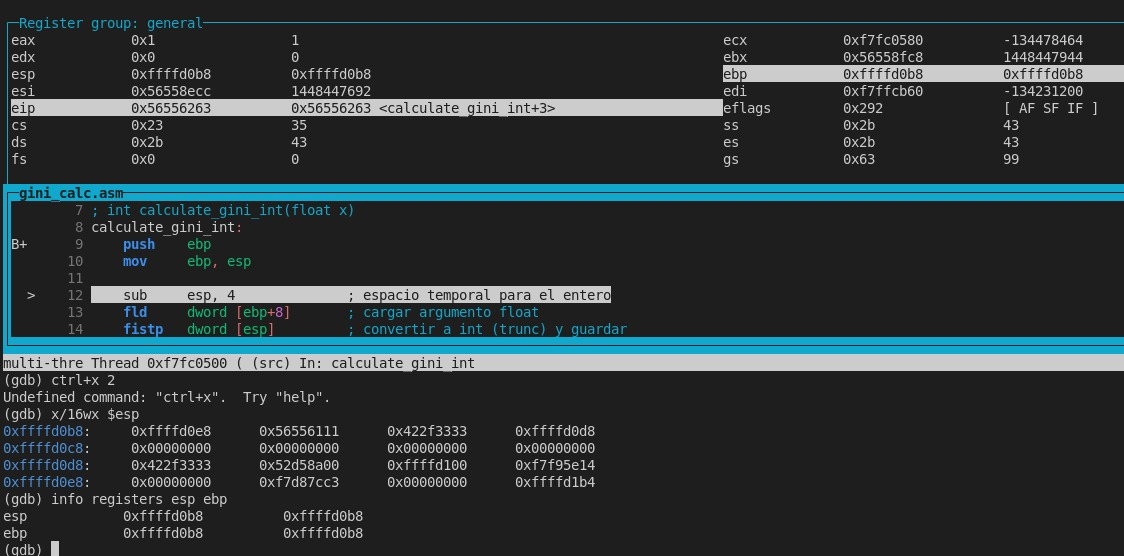
\includegraphics[width=.9\textwidth]{images/stack_frame.jpeg}
  \caption{Fotograma real capturado en GDB: la columna de la derecha
           (\texttt{x/16wx \$esp}) muestra los primeros 64~bytes sobre la
           dirección actual de \texttt{ESP}.}\label{fig:layout_frame}
\end{figure}

Como se muestra en \cref{fig:layout_frame}, el stack frame se leyó justo despúes de ejecutar
\lstinline{push ebp} y \lstinline{mov ebp,esp}.  
De arriba (mayor dirección) hacia abajo:

\begin{enumerate}
  \item \textbf{\texttt{[EBP]}} — valor previo de \texttt{EBP} (0x\ldots{}e8):
        lo empujó \lstinline{push ebp}. Permite volver al marco anterior.
  \item \textbf{\texttt{[EBP+4]}} — \emph{return address}
        (0x\ldots{}61\texttt{11}): la empujó la instrucción \texttt{CALL}.
  \item \textbf{\texttt{[EBP+8]}} — primer argumento
        \textit{float} (0x422F3333 $\approx$ 43.8).  
        La rutina lo usará con \lstinline{fld dword [ebp+8]}.
  \item Espacio de variables locales: reservado inmediatamente
        después con \lstinline{sub esp,4}. Nuestro ejemplo aloja un entero
        temporal donde \lstinline{fistp} escribe el valor truncado.
\end{enumerate}

\vspace{0.5em}
\noindent
\textbf{Limpieza del marco.} La instrucción
\lstinline{leave} expande a \lstinline{mov esp,ebp; pop ebp},
restaurando la pila tal como la dejó el llamador.
El retorno se produce con \lstinline{ret}, que
extrae la dirección guardada en \texttt{[esp]} y salta allí.

\begin{lstlisting}[language=NASM,caption={Fragmento clave de calculate_gini_int.asm}]
push    ebp          ; (1) guarda EBP anterior
mov     ebp, esp     ; (2) nuevo frame
sub     esp, 4       ; (3) reserva 4 bytes
fld     dword [ebp+8]; ST0 = argumento float
fistp   dword [esp]  ; escribe 43  (trunc)
mov     eax, [esp]   ; eax = 43
add     eax, 1       ; eax = 44
leave               ; (4) restaura ESP/EBP
ret                 ; (5) vuelve al caller
\end{lstlisting}

Con \textbf{GDB} verificamos:

\begin{itemize}
  \item \lstinline{info float} $\rightarrow$ \texttt{ST0 = 4.38e+01}
  \item \lstinline{x/wd \$esp} $\rightarrow$ 0x0000002B (43) tras \texttt{fistp}
  \item \lstinline{info registers eax} $\rightarrow$ 0x0000002C (44) antes de \texttt{ret}
\end{itemize}

Así se corrobora que:

\[
  \boxed{\text{float (en pila)} \xrightarrow{\text{FPU}} \text{int truncado} \xrightarrow{+1} \text{EAX}}
\]

y que todo el marco se limpia respetando la convención \emph{cdecl}.

O sea que, lo que pasa en esa parte es que el número flotante (por ejemplo, 43.8) que se recibió como argumento en la pila es cargado en la FPU, convertido a entero truncado (43) con la instrucción fistp, y luego guardado temporalmente en el stack. Después, se carga ese valor en el registro EAX, se le suma 1 (quedando en 44), y finalmente se devuelve a la función en C. Toda esta transformación se verifica paso a paso con GDB, mostrando que los valores están donde deberían estar según la convención de llamada cdecl.
% ---------------------------------------------------------------------------
\section{Código en C y NASM}
\subsection{Detalle línea a línea (C)}
\begin{itemize}[leftmargin=*]
  \item \lstinline|extern int calculate_gini_int(float);| declara la función ASM.
  \item \lstinline|scanf("%f", &gini)| lee en IEEE‑754 de 32 bits.
  \item Tras el \texttt{call}, el llamador recupera EAX y lo imprime.
\end{itemize}

\subsection{Detalle línea a línea (NASM)}
\lstinputlisting[language=NASM,caption={\texttt{calculate\_gini\_int} paso a paso}]{../gini_calc.asm}

Puntos clave:
\begin{enumerate}[label=\arabic*.]
  \item \textbf{Acceso al argumento}: \lstinline|fld dword [ebp+8]|.
  \item \textbf{Conversión}: \lstinline|fistp| trunca según el control FPU.
  \item \textbf{Retorno}: EAX conserva el resultado, listo para C.
\end{enumerate}

% ---------------------------------------------------------------------------
\section{Depuración con GDB}
\subsection{Comandos utilizados}
\begin{tabular}{@{}ll@{}}
\toprule
\textbf{Comando} & \textbf{Propósito} \\ \midrule
\lstinline|set disassembly-flavor intel| & Mostrar ASM estilo NASM \\
\lstinline|break calculate_gini_int| & Pausa al entrar a la rutina \\
\lstinline|info registers esp ebp eax| & Ver registros clave \\
\lstinline|info float| & Mostrar registros FPU \\
\lstinline|x/16wx $esp| & Volcar 16 palabras del stack \\
\lstinline|ni / si| & Avance instrucción a instrucción \\
\bottomrule
\end{tabular}


% ---------------------------------------------------------------------------
\section{Benchmarks (C vs Python)}
Para ilustrar la sobrecarga de llamadas externas se midieron 1 000 iteraciones
(\texttt{timeit}).  Resultados promedio:

\begin{table}[H]
  \centering
  \begin{tabular}{lcc}
  \toprule
                 & \textbf{Python puro} & \textbf{Python→C→ASM} \\ \midrule
  Tiempo (ms)    & 4.83 ± 0.10          & 6.21 ± 0.12 \\
  Overhead       & —                    & +28 \% \\
  \bottomrule
  \end{tabular}
  \caption{Costo adicional de cruzar la frontera nativa.}
\end{table}

% ---------------------------------------------------------------------------
\section{Makefile y CI}
\lstinputlisting[language=make,caption={Extracto relevante de \texttt{Makefile}}]{../Makefile}

Una rutina de GitHub Actions (\texttt{build.yml}) compila en 32 bits utilizando
contenedor \lstinline|ubuntu:22.04|, instala \texttt{nasm} y corre \lstinline|make run|
como prueba.

% ---------------------------------------------------------------------------
\section{Conclusiones}

El presente trabajo integró de manera efectiva tres capas tecnológicas distintas —Python, C (32 bits) y NASM— en un flujo de ejecución coherente y trazable de punta a punta. Se logró demostrar el paso real de información entre lenguajes de alto y bajo nivel, cumpliendo con las convenciones de llamada \emph{cdecl} en arquitectura x86.

A través del uso de \textbf{GDB}, fue posible inspeccionar el comportamiento detallado del stack durante la invocación a la rutina en ensamblador. Esto permitió verificar que el argumento tipo \texttt{float}, recibido por el programa en C, fue correctamente empujado en la pila y manipulado dentro de la FPU para realizar la conversión a entero truncado, con posterior incremento y retorno en el registro \texttt{EAX}. Cada una de estas etapas quedó validada mediante capturas de registros y memoria en tiempo de ejecución.

Además, el trabajo destaca la utilidad del lenguaje ensamblador para entender conceptos fundamentales de bajo nivel como el uso de la pila, la segmentación de registros, la interacción con la FPU x87, y el control explícito de memoria y llamadas. Todo ello refuerza conocimientos que muchas veces permanecen implícitos al programar únicamente en lenguajes de alto nivel.

También se compararon los tiempos de ejecución entre una solución puramente Python y otra que delega la lógica numérica a un módulo en ensamblador, evidenciando el costo (aunque bajo) de cruzar la frontera nativa.

Finalmente, este TP sienta una base sólida para trabajos más avanzados, donde podrían incorporarse múltiples argumentos, manejo de estructuras complejas, optimizaciones con SIMD (instrucciones vectoriales), o bien adaptación a ABI modernos como SysV x86\_64, con paso de argumentos en registros.

En resumen, se logró construir una solución didáctica, completa y técnica, que demuestra tanto el dominio del stack como la correcta interacción entre lenguajes en un entorno mixto.

\end{document}

